\begin{frame}
  \frametitle{\textbf{QGP at Particle Colliders}}
  \begin{itemize}
  \item We can create QGP in the lab by colliding heavy nuclei ($v \approx c$) in particle accelerators (such as RHIC and LHC)
  \item QCD predicts rich phase dynamics prior to particle detection
    \begin{itemize}
    \item \textbf{Strongly-interacting QGP phase} that flows as a relativistic hydrodynamic fluid
    \item Medium expansion, cooling, and \textbf{hadronization}
    \item Hadronic rescattering and \textbf{freeze-out}
    \end{itemize}
  \end{itemize}

  \
  
  \centering
  \begin{tikzpicture}
    \node{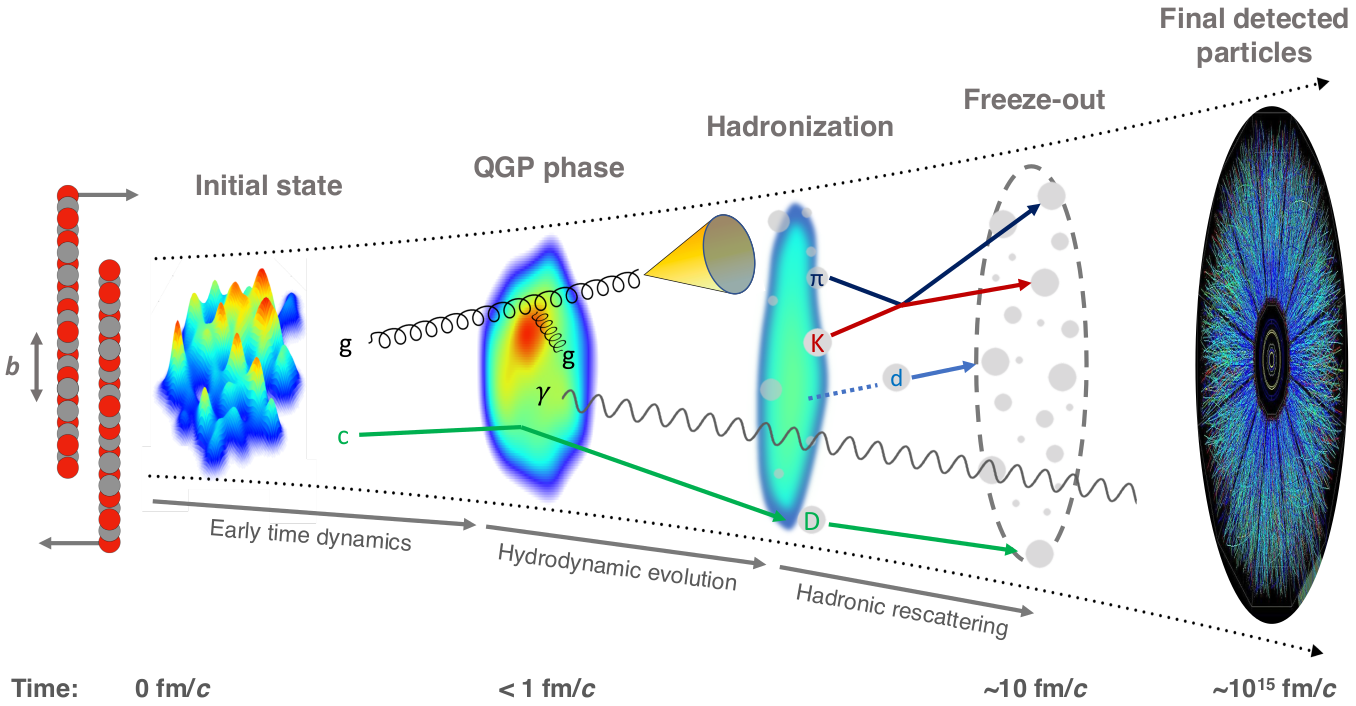
\includegraphics[width=0.8\textwidth]{collision-stages.png}};
  \end{tikzpicture}
\end{frame}
